\documentclass[11pt,a4paper]{article}
\usepackage[T1]{fontenc}\usepackage[utf8]{inputenc}\usepackage{lmodern,microtype}
\usepackage{amsmath,amssymb,amsthm,mathtools,bm}
\usepackage{booktabs,array,tabularx,longtable,multirow}
\usepackage{graphicx,float,caption,xcolor}
\usepackage[margin=22mm]{geometry}\usepackage{enumitem,fancyhdr,hyperref,pdflscape}
\definecolor{finblue}{HTML}{1F5A99}\definecolor{fingreen}{HTML}{19733A}\definecolor{finorange}{HTML}{C45A00}\definecolor{finred}{HTML}{A61B1B}\definecolor{fingray}{HTML}{4E5964}\definecolor{finsoft}{HTML}{F2F5F8}
\hypersetup{colorlinks=true,linkcolor=finblue,urlcolor=finblue,citecolor=fingreen,pdftitle={FIN ST552--ST641: Refinement-Speed No-Go, Conditional Light Cone, and Two-Clock Continuum},pdfauthor={Krzysztof Żuchowski},pdfsubject={Six local FIN research rounds on layer-covariant propagation and causality},pdfkeywords={FIN, nadsoliton, speed of light, refinement, causal cone, dispersion, dual dynamics, continuum limit, no-go theorem}}
\pagestyle{fancy}\fancyhf{}\fancyhead[L]{\small FIN ST552--ST641}\fancyhead[R]{\small Release 10.90}\fancyfoot[C]{\thepage}\setlength{\headheight}{14pt}
\newtheorem{theorem}{Theorem}[section]\newtheorem{proposition}[theorem]{Proposition}\newtheorem{corollary}[theorem]{Corollary}
\theoremstyle{remark}\newtheorem{remark}[theorem]{Remark}
\newcommand{\R}{\mathbb R}\newcommand{\Z}{\mathbb Z}\newcommand{\one}{\bm1}\newcommand{\Tr}{\operatorname{Tr}}
\newcommand{\status}[2]{\textcolor{#1}{\textbf{[#2]}}}\newcommand{\proven}{\status{fingreen}{PROVEN}}\newcommand{\strong}{\status{finblue}{STRONG EVIDENCE}}\newcommand{\conditional}{\status{fingray}{CONDITIONAL}}\newcommand{\open}{\status{finorange}{OPEN}}\newcommand{\blocked}{\status{finred}{BLOCKED}}
\newcommand{\claimbox}[1]{\begin{center}\fcolorbox{finblue}{finsoft}{\parbox{.92\textwidth}{#1}}\end{center}}
\setlist[itemize]{leftmargin=*,itemsep=2pt,topsep=3pt}\setlist[enumerate]{leftmargin=*,itemsep=2pt,topsep=3pt}\setlength{\emergencystretch}{2em}

\begin{document}\hypersetup{pageanchor=false}
\begin{titlepage}\centering\vspace*{14mm}{\Huge\bfseries FIN ST552--ST641\par}\vspace{4mm}
{\Large Refinement-Speed No-Go, Conditional Light-Cone Emergence,\par}{\Large and the Two-Clock Continuum Architecture\par}\vspace{12mm}
{\Large Krzysztof Żuchowski\par}{\normalsize Independent Researcher --- Fractal Information Theory Project\par}{\normalsize ORCID: 0009-0002-0909-3613\par}\vspace{9mm}
{\large Six consecutive research rounds\par}{\large FIN Release 10.90 --- Version 1.0.0\par}{\large 30 August 2026\par}\vfill
\begin{minipage}{.91\textwidth}\small
\textbf{Scope.} This report studies whether FIN can generate a layer-invariant propagation speed or causal cone from its strict twelve-state operator and exact refinement results. It includes ST552--ST641 only and preserves the legacy/strict kernel split.

\medskip\textbf{Evidence boundary.} All results are analytic, exact finite-dimensional, interval, or explicitly numerical within declared models. No physical light field, laboratory clock, ruler, detector record or independent external audit is supplied.

\medskip\textbf{Repository.} \url{https://github.com/hyconiek/Fractal-Nadsoliton-Theory}\qquad\textbf{License.} CC BY 4.0.
\end{minipage}\vfill\end{titlepage}\hypersetup{pageanchor=true}

\begin{abstract}
Six consecutive FIN research rounds investigate the hypothesis that internal observers on different fractal/refinement layers may reconstruct the same propagation speed even when their local length and time standards differ. The correct layer law is
\[
c_n^{\rm phys}=\frac{\ell_n}{\tau_n}\widehat c_n,
\qquad
\frac{c_{n+1}^{\rm phys}}{c_n^{\rm phys}}
=\frac{\alpha_n}{\beta_n}\frac{\widehat c_{n+1}}{\widehat c_n}.
\]
Equal length/time scaling is sufficient only when the dimensionless dispersion slope is itself refinement invariant.

For the fixed strict $C_{12}$ operator, a formal continuous-symbol slope $\widehat c=1.9015886526$ can be computed, but the first available discrete mode has phase and group speeds $1.65852$ and $1.22656$, and the full radial graph has no exact causal cone. Candidate refinements separate into inequivalent universality classes. A paired finite-range continuation has quadratic low-wave-number symbol and speed $1.9532829072$. A positive $d^{-1.8}$ tail has fractional symbol order $0.8$, wave exponent $0.4$ and divergent low-$k$ group speed. The literal signed oscillatory strict continuation loses positive-semidefinite Laplacian structure already at the tested carrier $N=48$.

The central no-go theorem comes from the exact dyadic refinement fiber. For every $q\ge0$, $A_{24}(q)J=JA_{12}$ and all coarse unitary and heat records are identical, while the fine formal speed obeys
\[
\widehat c(q)^2=\widehat c(0)^2+72q.
\]
Thus complete coarse dynamics is exactly compatible with a continuous unbounded family of fine speeds. Across a tower,
\[
C_{2N}=C_N+\frac{N^2}{2}q_N.
\]
A finite infinite-depth speed requires $\sum N^2q_N<\infty$; a uniform exponential propagation bound requires exponential rather than polynomial decay of antipodal rates. Exact speed or trace-density stationarity conditionally selects $q_N=0$, but neither stationarity law is strict-sourced.

For the conditional zero-rate finite-range tower on a fixed physical circle, $A_N/a_N^2$ converges to $-C\partial_x^2$. A scalar $1+1$ wave equation with an exact limiting domain of dependence therefore emerges conditionally, and numerical finite-lattice tails outside $1.05\widehat c t$ fall to $8.2\times10^{-9}$ by $N=12288$. However, one universal refinement clock is impossible: unitary/heat limits require $t\sim a^{-2}$ while the second-order wave channel requires $t\sim a^{-1}$. Two channel-specific clock classes and a dimensional length/time anchor remain necessary. FIN therefore permits a coherent emergent-cone completion but does not make it inevitable, does not derive the SI value of $c$, and does not yet supply Lorentzian $3+1$ spacetime or physical light.
\end{abstract}

\noindent\textbf{Claim vocabulary.} \proven{} means an analytic/exact/interval theorem in scope; \strong{} means reproducible nonexhaustive numerical evidence; \conditional{} requires displayed additional premises; \open{} is unresolved; \blocked{} denotes a missing typed input, not a refutation of all future completions.
\tableofcontents\newpage

\section{Executive synthesis}
\claimbox{\textbf{Main result.} The current strict endpoint and exact coarse-refinement axioms do not determine a propagation speed. They admit infinitely many fine generators with identical complete coarse spectral dynamics and arbitrarily different fine speed/locality data. A conditional local continuum with a wave cone exists only after choosing a zero-rate finite-range tower, coordinate scaling, a ballistic wave clock and dimensional calibration.}

\begin{table}[H]\centering\caption{Central status map.}\small\begin{tabularx}{\textwidth}{@{}p{.25\textwidth}X p{.21\textwidth}@{}}\toprule Question&Answer&Status\\\midrule
Does $A_{12}$ define a physical $c$?&It defines finite dimensionless proxies, not a continuum slope or SI speed.&\blocked\\
Does the full strict graph have an exact cone?&No; opposite vertices are directly coupled.&\proven\\
Which tail permits finite low-$k$ speed?&Exactly a quadratic symbol $\lambda\sim Ck^2$.&\proven\\
Does $d^{-1.8}$ give that symbol?&A positive envelope has order $0.8$, hence divergent group speed.&\proven\\
Does exact refinement select a speed?&No; the $q$ fiber preserves all coarse records but changes fine speed.&\proven\\
Can a conditional local limit exist?&Yes, for the added zero-rate finite-range tower with $A_N/a_N^2$.&\conditional\\
Can one clock preserve all channels?&No; $U/P$ need $a^{-2}$ and the wave channel needs $a^{-1}$.&\proven\\
Is physical light derived?&No; $3+1$ geometry, boosts, gauge structure and calibration remain missing.&missing\\\bottomrule\end{tabularx}\normalsize\end{table}

The strongest scientific conclusion is a distinction between \emph{compatibility} and \emph{inevitability}. FIN is compatible with a local wave completion. Current FIN does not select it over fractional, signed or nonlocal refinements.

\section{Frozen strict core and channel definitions}
On $C_{12}$ define
\[
W_{xx}=0,\qquad W_{xy}=K_{\rm strict}(d(x,y)),\qquad A=sI-W,
\]
with
\[
K_{\rm strict}(d)=\frac{\cos(0.18575d+0.16250)}{1+d^{1.8}}.
\]
The strict weights at distances $1$ through $6$ are positive and $A\succeq0$. Three spectral calculi are kept distinct:
\[
U_t=e^{-itA},\qquad P_t=e^{-tA},\qquad C_t=\cos(t\sqrt A).
\]
$U_t$ and $P_t$ use the eigenvalue $\lambda$ as phase frequency/decay rate; the second-order wave channel uses $\sqrt\lambda$. Common projectors do not imply common dimensional time maps.

For a continuous interpolation of the finite symbol,
\[
\lambda_{12}(q)=2\sum_{d=1}^{5}w_d(1-\cos dq)+w_6(1-\cos6q),
\]
the formal coefficient is
\[
\widehat c_{12}^2=\sum_{d=1}^{5}w_dd^2+18w_6,
\qquad \widehat c_{12}=1.9015886526.
\]
Yet $q_{\min}=\pi/6$, so $C_{12}$ contains no actual $q\to0$ sequence.

\section{Round I: ST552--ST566}
\subsection{Speed proxy and causal obstruction}
The first strict mode gives
\[
v_{\rm phase}=1.6585246837,
\qquad v_{\rm group}=1.2265636961,
\]
well separated from the formal tangent. The full graph directly couples every cyclic distance, so the unitary Born probability at the opposite site begins as $O(t^2)$ and heat probability as $O(t)$. No strict finite cone is present.

\begin{figure}[H]\centering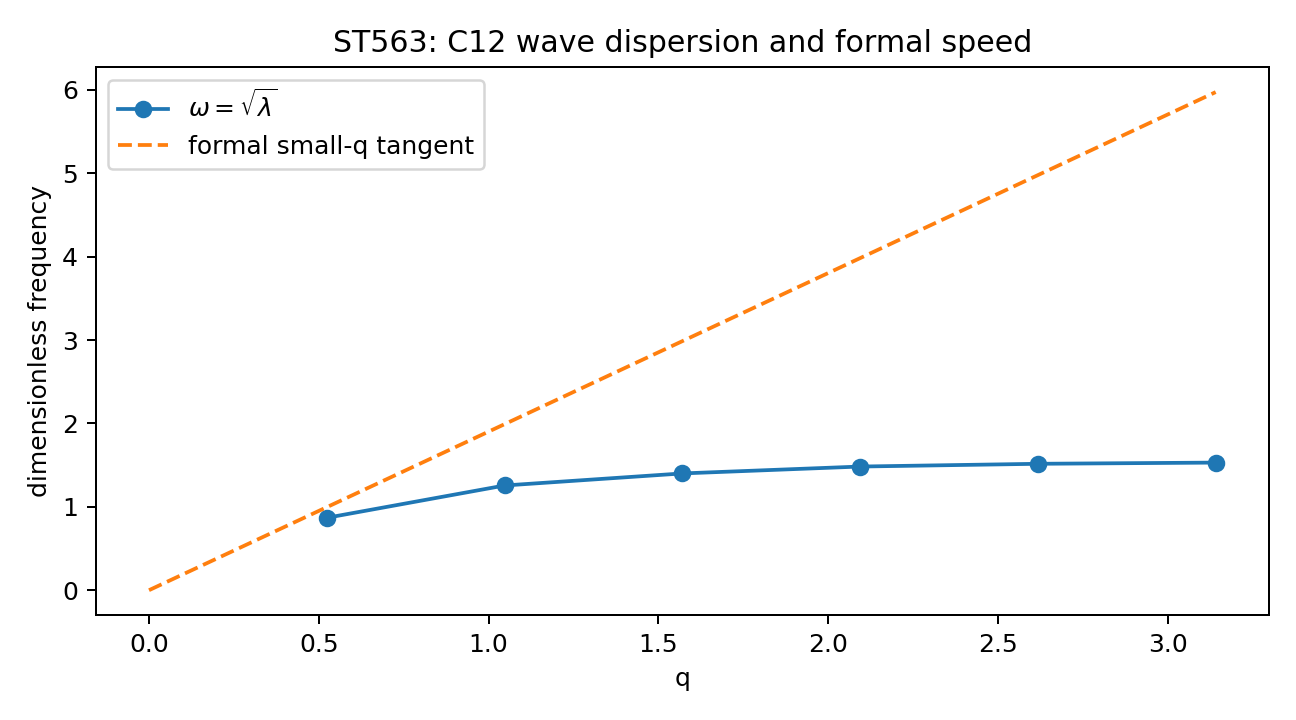
\includegraphics[width=.82\textwidth]{FIN_ST552_ST566_Figures/st563_dispersion.png}\caption{Finite $C_{12}$ dispersion and its formal tangent. The tangent is not an available physical mode.}\end{figure}

Layer covariance requires
\[
\boxed{\frac{\alpha_n}{\beta_n}\frac{\widehat c_{n+1}}{\widehat c_n}=1.}
\]
The frequently proposed condition $\alpha_n=\beta_n$ is sufficient only if $\widehat c_{n+1}=\widehat c_n$, which is precisely the missing refinement theorem.

\subsection{Other Round-I frontiers}
The 38-relation degree-eight block again failed rational reconstruction after a conditioned five-prime lift, so no characteristic-zero rank was promoted. The first-transition orbit remained globally open. A CPTP operational-conjugacy fixture passed with trace-preservation residuals below $1.5\times10^{-14}$. IR interval continuation reached $b=0.2592$ before radius inflation became method-gated.

\subsection{Round-I ledger}
\begin{longtable}{@{}p{.09\textwidth}p{.32\textwidth}p{.49\textwidth}@{}}\toprule Program&Status&Result\\\midrule\endhead
ST552--556&open/gated&Conditioned 38-relation lift still fails rational reconstruction.\\
ST557--559&\strong&Two-level/reflection searches support the candidate transition; globality open.\\
ST560&\proven&Equivariant irreducible Markov selector is uniform.\\
ST561&\strong&Synthetic three-channel finite-shot classifier passes 1\% target.\\
ST562&\proven&CPTP operational conjugacy fixture.\\
ST563&\proven&Finite speed proxies and exact-cone obstruction.\\
ST564&\proven&IR continuation reaches $b=0.2592$.\\
ST565--566&blocked&No physical cone, speed source or evidence.\\\bottomrule\end{longtable}

\section{Round II: ST567--ST581}
\subsection{Three inequivalent refinements}
For a paired finite-range continuation,
\[
\lambda(q)=2\sum_{d=1}^{6}w_d(1-\cos dq)
=Cq^2+O(q^4),\qquad
C=\sum_{d=1}^{6}w_dd^2,
\]
and
\[
\widehat c_{\rm FR}=\sqrt C=1.9532829072.
\]
The first-mode slopes converge to this number as $N\to\infty$.

\begin{figure}[H]\centering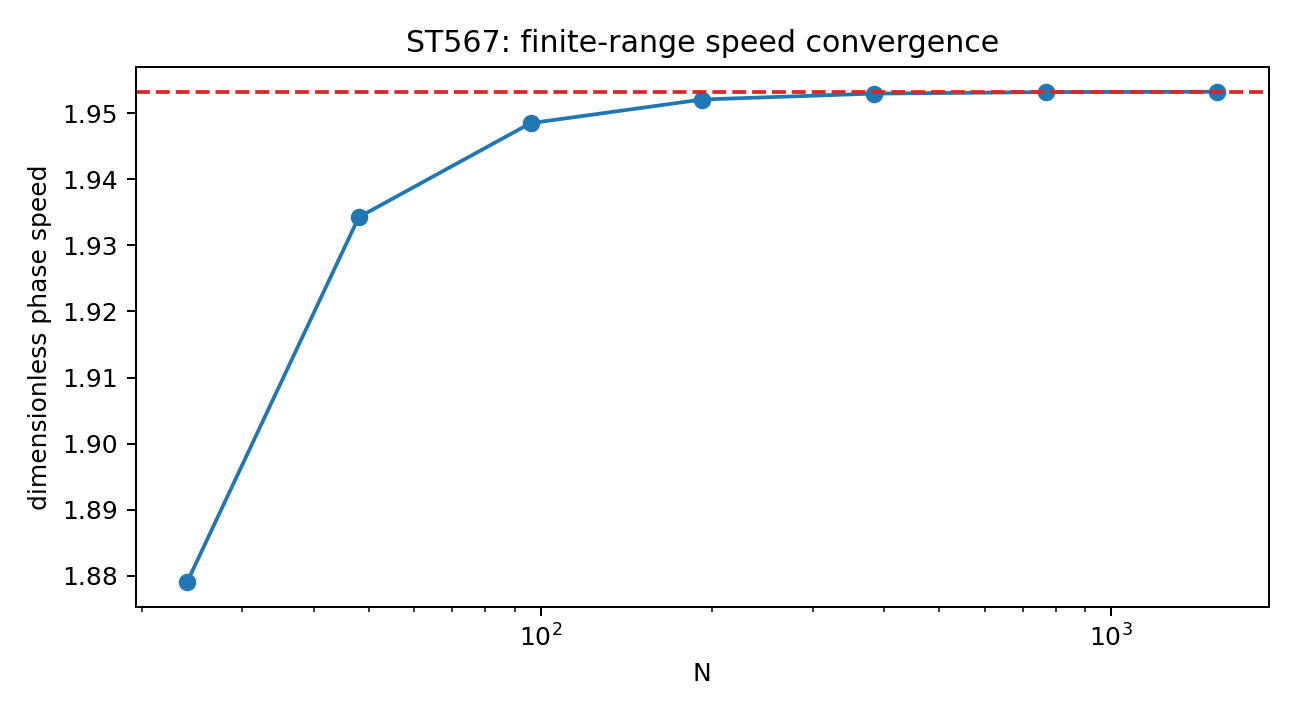
\includegraphics[width=.8\textwidth]{FIN_ST567_ST581_Figures/st567_finite_speed.png}\caption{Conditional finite-range phase-speed convergence.}\end{figure}

For the positive envelope $a_d=(1+d^{1.8})^{-1}$, the fitted low-$q$ symbol exponent is $0.7970$, consistent with $\eta-1=0.8$. Hence $\omega\sim|q|^{0.4}$ and $v_g\sim|q|^{-0.6}$.

\begin{figure}[H]\centering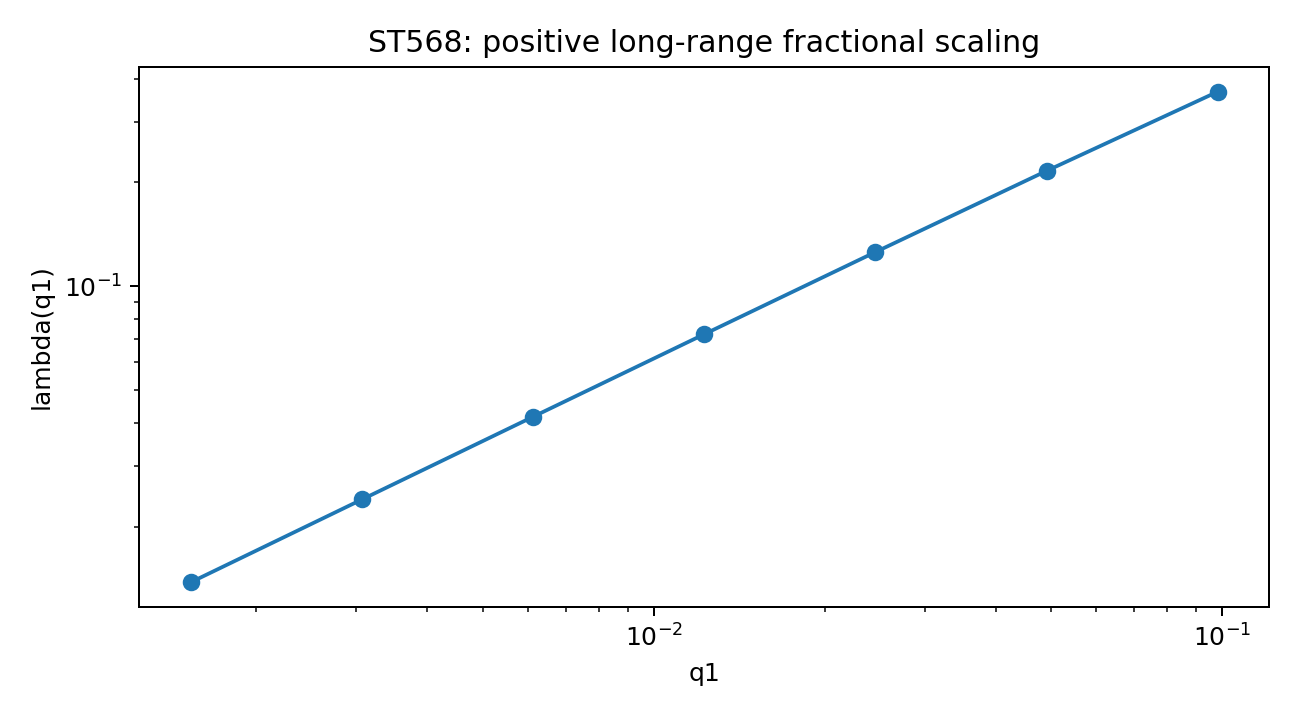
\includegraphics[width=.8\textwidth]{FIN_ST567_ST581_Figures/st568_fractional.png}\caption{Positive long-range envelope: fractional rather than quadratic scaling.}\end{figure}

The literal oscillatory strict formula, extended to all distances, introduces negative weights and negative Laplacian modes at tested $N=48$.

\begin{figure}[H]\centering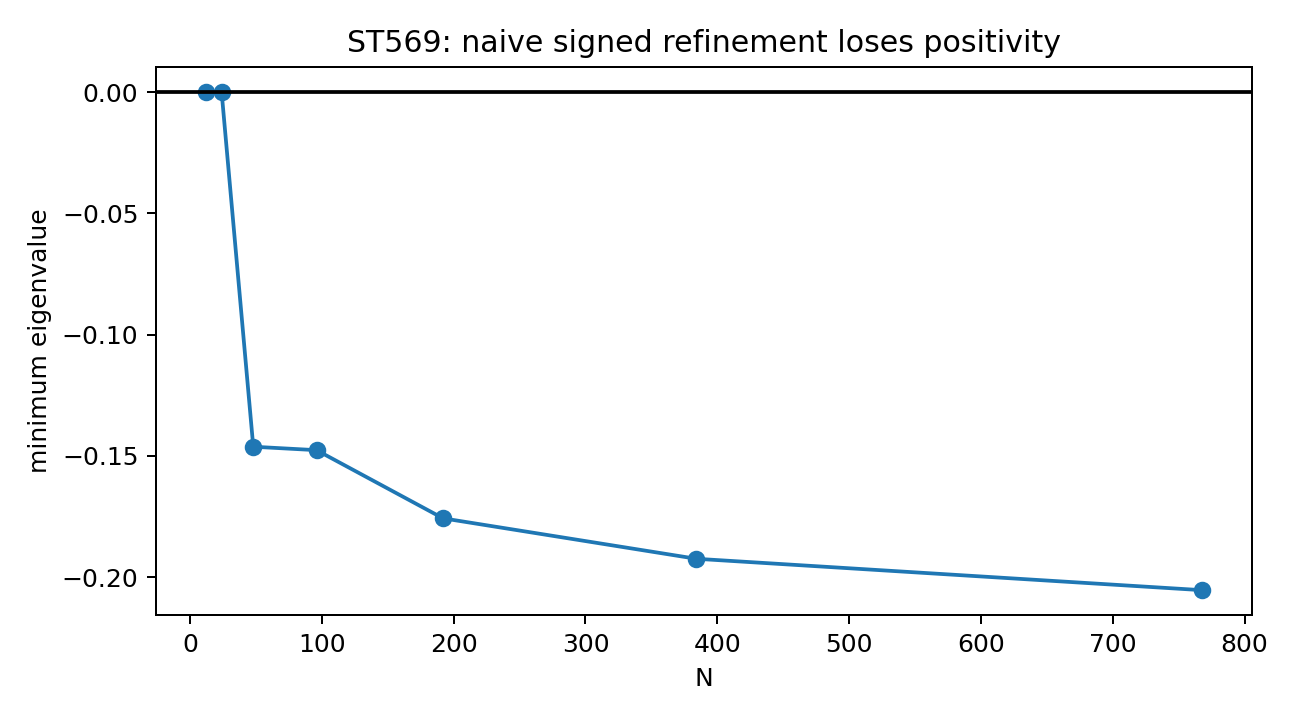
\includegraphics[width=.8\textwidth]{FIN_ST567_ST581_Figures/st569_signed_no_go.png}\caption{Naive signed strict refinement loses positive-semidefinite generator structure.}\end{figure}

Thus $A_{12}$ admits mutually incompatible continuations: local/quadratic, positive/fractional and signed/indefinite.

\subsection{Locality and chart results}
The finite-range exponential-moment velocity proxy is $3.00711$, while the maximal sampled wave group velocity is $1.95328$. This is an approximate single-particle cone, not Lorentz invariance. A logarithmic IR chart reduced numerical Jacobian conditioning by a median factor $35.4$, but the interval implementation was not yet certified.

\subsection{Round-II ledger}
\begin{longtable}{@{}p{.09\textwidth}p{.32\textwidth}p{.49\textwidth}@{}}\toprule Program&Status&Result\\\midrule\endhead
ST567&\proven&Finite-range quadratic dispersion limit.\\
ST568&\strong&Positive long-range fractional exponent $\approx0.8$.\\
ST569&\proven&Finite counterexample to naive positive signed refinement.\\
ST570&\proven&Layer-speed covariance depends on refinement.\\
ST571&conditional&Finite-range LR velocity proxy.\\
ST572--573&\proven&Spectrum/speed coordinate distinction and short-time tails.\\
ST574--577&gated&Transition interval and characteristic-zero methods remain open.\\
ST578&\conditional&Three-channel noise scaling.\\
ST579&\strong&Log-chart floating conditioning improved.\\
ST580--581&blocked&No physical $c$, Lorentz cone or evidence.\\\bottomrule\end{longtable}

\section{Round III: ST582--ST596}
\subsection{Dispersion theorem}
\begin{theorem}[Positive-tail symbol]
If $a_d\sim c d^{-1-\alpha}$ with $0<\alpha<2$, then
\[
2\sum_{d\ge1}a_d(1-\cos kd)
\sim2cI_\alpha|k|^\alpha,
\quad
I_\alpha=\frac{\pi}{2\Gamma(1+\alpha)\sin(\pi\alpha/2)}.
\]
\end{theorem}
For $\alpha=0.8$, $2I_\alpha=3.5466218138$.

\begin{theorem}[Speed trichotomy]
If $\lambda(k)\sim C|k|^\nu$, then
\[
v_g(k)\sim\sqrt C\frac\nu2|k|^{\nu/2-1}.
\]
A finite nonzero low-$k$ speed exists if and only if $\nu=2$.
\end{theorem}

\begin{figure}[H]\centering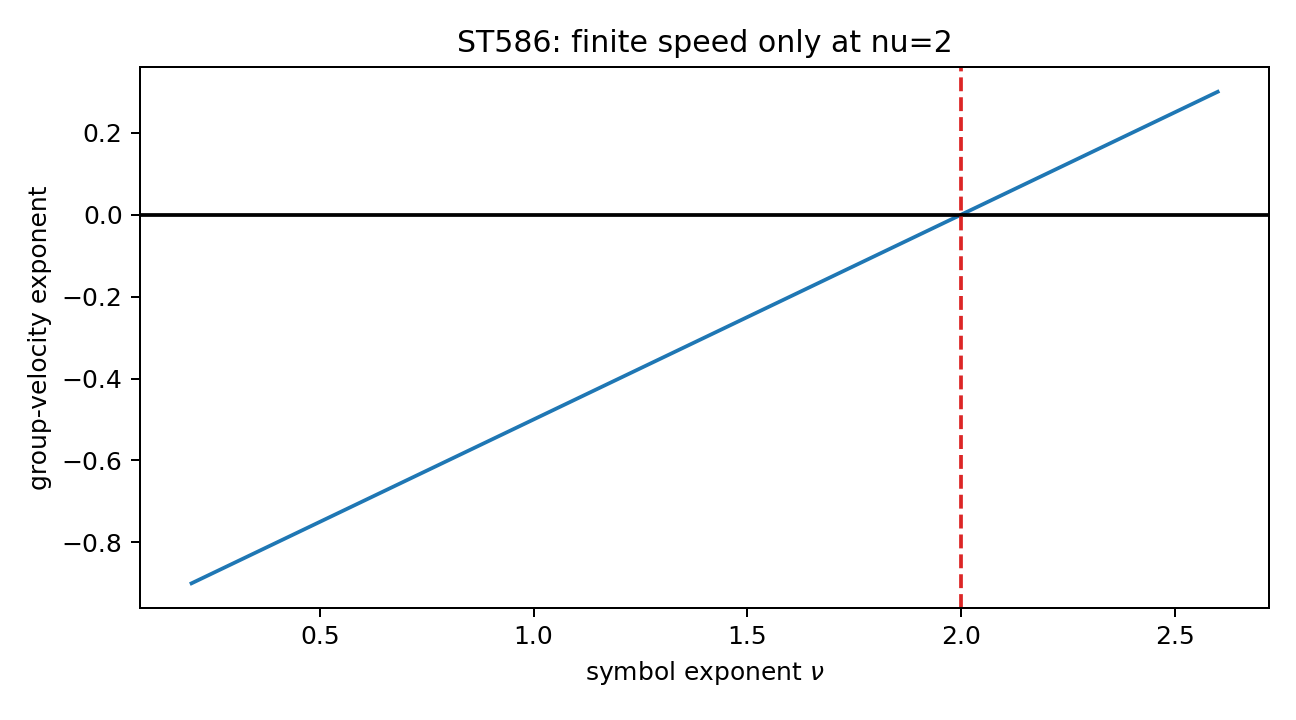
\includegraphics[width=.78\textwidth]{FIN_ST582_ST596_Figures/st586_speed_trichotomy.png}\caption{Only a quadratic generator symbol yields a finite nonzero massless speed.}\end{figure}

For finite range, exponential conjugation gives the single-particle bound
\[
|\langle x|e^{-itA}|y\rangle|
\le e^{-\mu(r-v_\mu|t|)},
\qquad
v_\mu=\frac{2}{\mu}\sum_dw_d\sinh(\mu d).
\]
Long-range direct couplings instead give immediate polynomial spatial tails.

\subsection{Honest IR failure}
Direct interval substitution $x=e^z$ inflated dependencies. The first proposed log Krawczyk cell has margin $-0.00663$ and is rejected. No log interval chain or degree theorem is claimed. This is a bounded no-go for the naive chart, not disappearance of the numerical root.

\subsection{Round-III ledger}
\begin{longtable}{@{}p{.09\textwidth}p{.32\textwidth}p{.49\textwidth}@{}}\toprule Program&Status&Result\\\midrule\endhead
ST582--584&bounded stop&Naive log interval chart rejected; no degree promotion.\\
ST585&\proven&Positive-tail fractional-symbol theorem.\\
ST586&\proven&Dispersion-exponent speed trichotomy.\\
ST587--589&\proven&Finite-range cone bound, tail classification and scale torsor.\\
ST590&\conditional&Dimensionless speed estimator.\\
ST591--593&gated&Transition/reflection/algebra methods frozen.\\
ST594--596&blocked&No seed/gain/selector, physical $c$ or evidence.\\\bottomrule\end{longtable}

\section{Round IV: ST597--ST611}
\subsection{Exact speed fiber and observer blindness}
The known exact dyadic family satisfies
\[
A_{24}(q)J=JA_{12},\qquad q\ge0.
\]
Its even modes and every coarse spectral function are independent of $q$, while
\begin{equation}\label{eq:speedfiber}
\boxed{\widehat c(q)^2=\widehat c(0)^2+72q.}
\end{equation}
For $q=0,0.1,1$, the formal speeds are $1.90159$, $3.28877$ and $8.69575$, while coarse generator/unitary/heat residuals remain below $2\times10^{-15}$.

\begin{figure}[H]\centering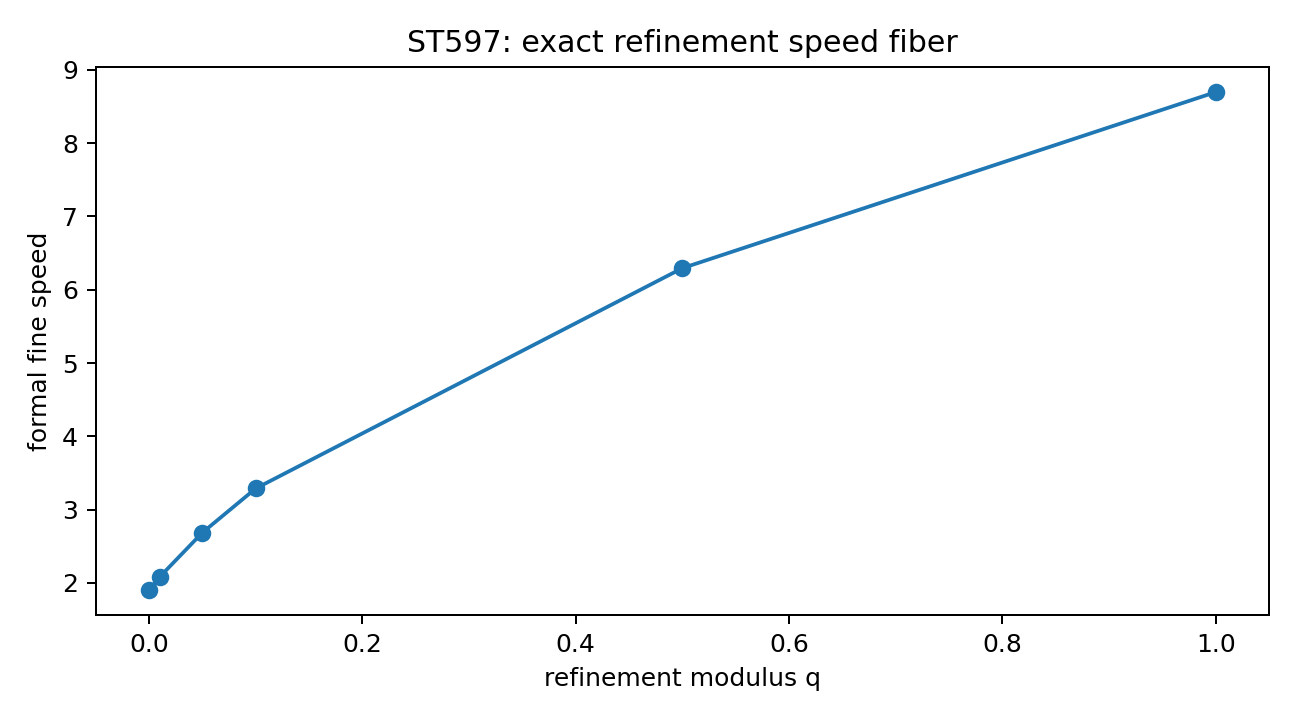
\includegraphics[width=.8\textwidth]{FIN_ST597_ST611_Figures/st597_speed_fiber.png}\caption{A continuous unbounded fine-speed fiber with identical complete coarse dynamics.}\end{figure}

\begin{theorem}[Coarse speed nonidentifiability]
No observable constructed solely from complete coarse spectral dynamics identifies $q$ or the fine speed in \eqref{eq:speedfiber}.
\end{theorem}
A single child-resolved odd Fourier mode recovers $q$ because every odd eigenvalue shifts by exactly $2q$.

Trace-density conservation conditionally selects $q=0$, but this is an added refinement axiom. Unlabelled-fiber naturality similarly leaves a vertical sector rate $v\ge0$ invisible to coarse dynamics.

\subsection{Round-IV ledger}
\begin{longtable}{@{}p{.09\textwidth}p{.32\textwidth}p{.49\textwidth}@{}}\toprule Program&Status&Result\\\midrule\endhead
ST597&\proven&Exact speed fiber $\widehat c^2=C+72q$.\\
ST598&\proven&Complete coarse observer is blind to fine speed.\\
ST599&\proven&Antipodal-rate speed-scaling trichotomy.\\
ST600&\conditional&Trace stationarity selects $q=0$.\\
ST601--602&\proven&Hidden vertical sector and fine tomography of $q$.\\
ST603--605&\proven&Calibration compensation, locality cost and canonical-speed no-go.\\
ST606--608&open/gated&Transition, algebra and IR predictor chart obligations.\\
ST609&\proven&Dual dynamics does not derive propagation speed.\\
ST610--611&blocked&No physical speed/source/evidence closure.\\\bottomrule\end{longtable}

\section{Round V: ST612--ST626}
\subsection{Multilevel speed recurrence}
For a dyadic tower with parent size $N$ and new antipodal rate $q_N$,
\begin{equation}\label{eq:recurrence}
\boxed{C_{2N}=C_N+\frac{N^2}{2}q_N.}
\end{equation}
Hence
\[
C_j=C_0+\frac12\sum_{i<j}N_i^2q_i.
\]
For nonnegative rates, a finite infinite-depth speed exists exactly when
\[
\sum_iN_i^2q_i<\infty.
\]
The often suggested law $q_N\sim\kappa N^{-2}$ adds $\kappa/2$ per layer and therefore diverges linearly with depth. Exact speed stationarity forces $q_N=0$ at every layer.

Uniform exponential locality is stricter: a fixed exponential moment requires $q_N\sinh(\mu N)$ bounded. Every polynomial $N^{-p}$ fails; exponential distance decay is necessary within this bound architecture.

\begin{figure}[H]\centering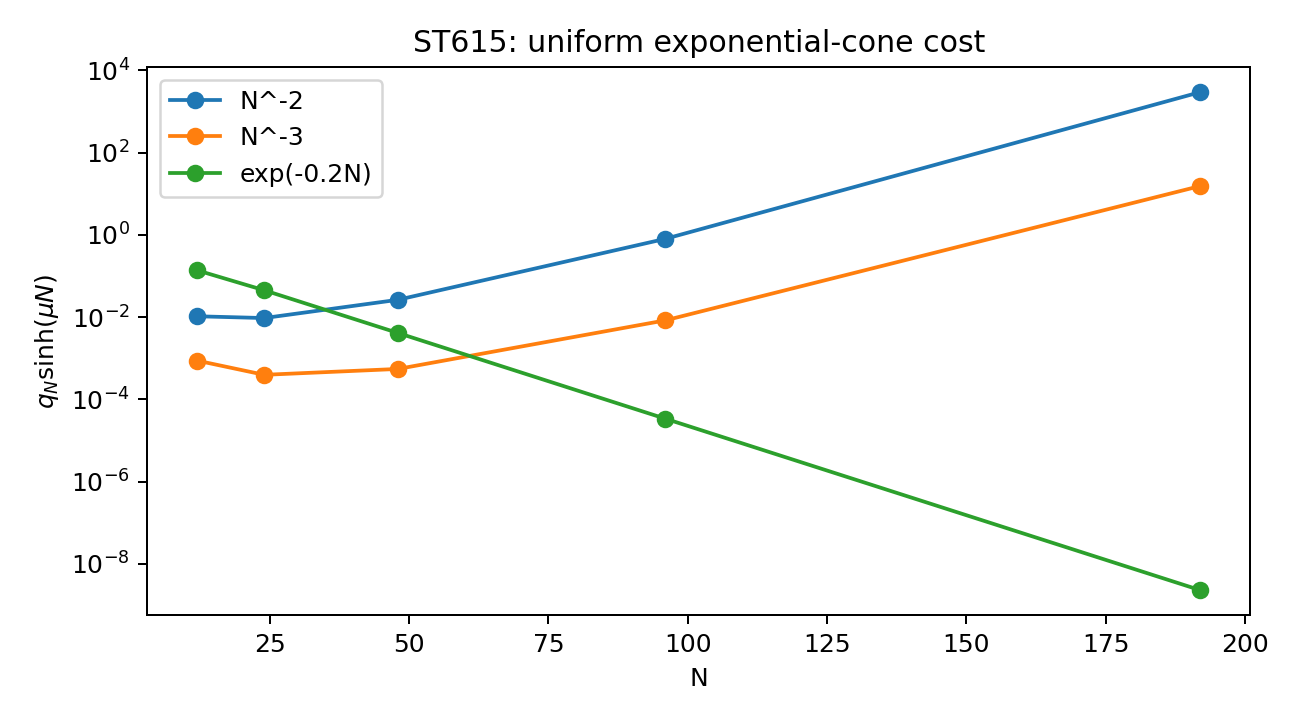
\includegraphics[width=.8\textwidth]{FIN_ST612_ST626_Figures/st615_locality_scaling.png}\caption{Polynomial antipodal rates fail a uniform exponential locality cost.}\end{figure}

Two depth-three towers with final formal speeds $1.90159$ and $4.47572$ have identical base generator and heat records below $1.2\times10^{-15}$. Coassociativity does not constrain the one new rate per level. Each rate is nevertheless exactly recoverable by a child-resolved odd mode.

\subsection{Round-V ledger}
\begin{longtable}{@{}p{.09\textwidth}p{.32\textwidth}p{.49\textwidth}@{}}\toprule Program&Status&Result\\\midrule\endhead
ST612--614&\proven&Speed recurrence, convergence criterion and conditional zero tower.\\
ST615&\proven&Polynomial antipodal rates fail a uniform exponential cone.\\
ST616--617&\proven&Multilevel coarse blindness and level tomography.\\
ST618--619&\proven&Rate-record complexity and coassociativity no-selection.\\
ST620--621&\proven&Trace/speed laws share zero solution but remain inequivalent; calibration compensation.\\
ST622&\conditional&Zero-rate quadratic-symbol continuum candidate.\\
ST623&\proven&Refinement universality classes separated.\\
ST624--626&blocked&No rate source, physical continuum or evidence.\\\bottomrule\end{longtable}

\section{Round VI: ST627--ST641}
\subsection{One-clock no-go}
Let $a_N=L/N$ and keep physical wave number $k$ fixed. The zero-rate finite-range symbol satisfies
\[
\lambda_N(a_Nk)=Ca_N^2k^2+O(a_N^4k^4).
\]
Thus:
\[
t_U,t_H\sim a_N^{-2},\qquad t_W\sim a_N^{-1}.
\]

\begin{theorem}[Single-clock no-go]
No single power-law clock $t\sim a^{-z}$ produces simultaneous nontrivial unitary/heat and second-order wave limits. The first pair requires $z=2$, the wave channel requires $z=1$.
\end{theorem}
The minimal architecture contains one diffusive/Schrödinger clock class and one ballistic wave-clock class. Their absolute normalizations remain free.

\subsection{Conditional continuum bridge}
For the added zero-rate finite-range tower,
\[
\frac{A_N}{a_N^2}\longrightarrow-C\partial_x^2,
\qquad C=3.8153141155,
\qquad\widehat c=\sqrt C=1.9532829072.
\]
The consistency error is $O(a_N^2)$ and controlled by the finite fourth moment $52.4176613$.

\begin{figure}[H]\centering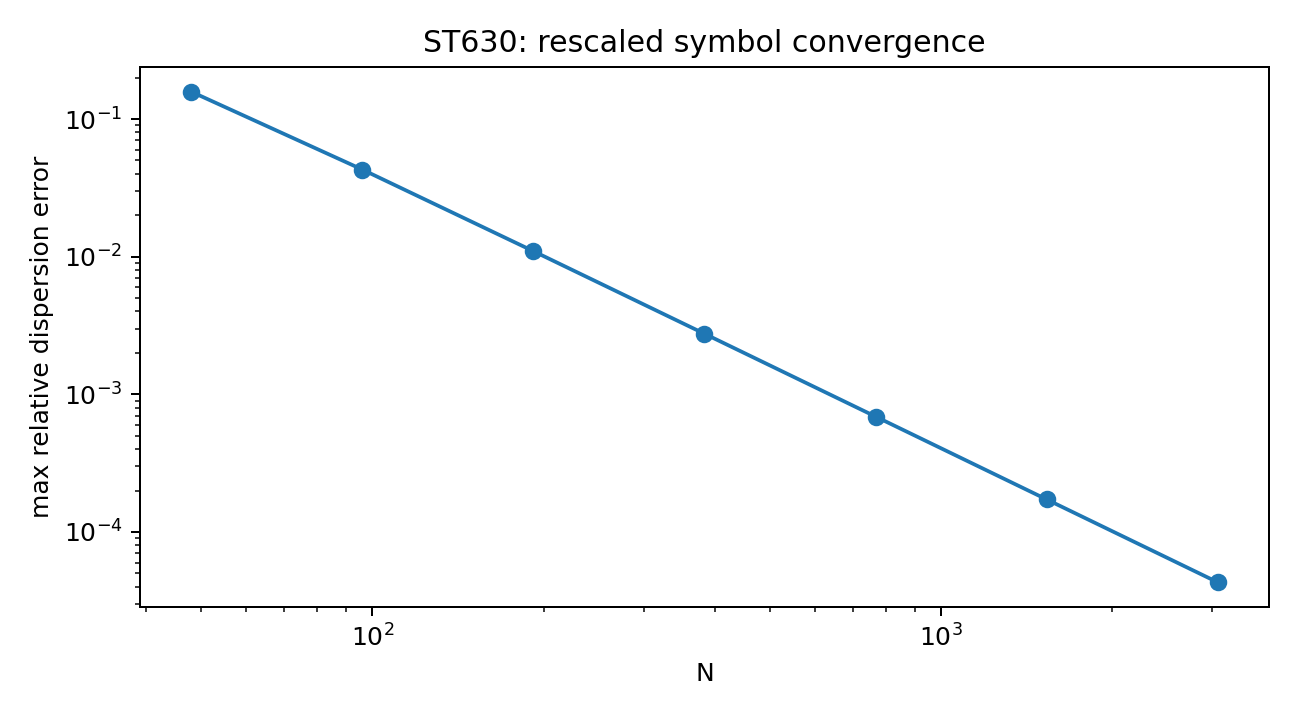
\includegraphics[width=.8\textwidth]{FIN_ST627_ST641_Figures/st630_dispersion_convergence.png}\caption{Convergence of the first three rescaled physical modes to $Ck^2$.}\end{figure}

For a localized displacement at physical time $T=0.5$, the relative finite-lattice tail beyond $1.05\widehat cT$ decreases to $8.20\times10^{-9}$ at $N=12288$.

\begin{figure}[H]\centering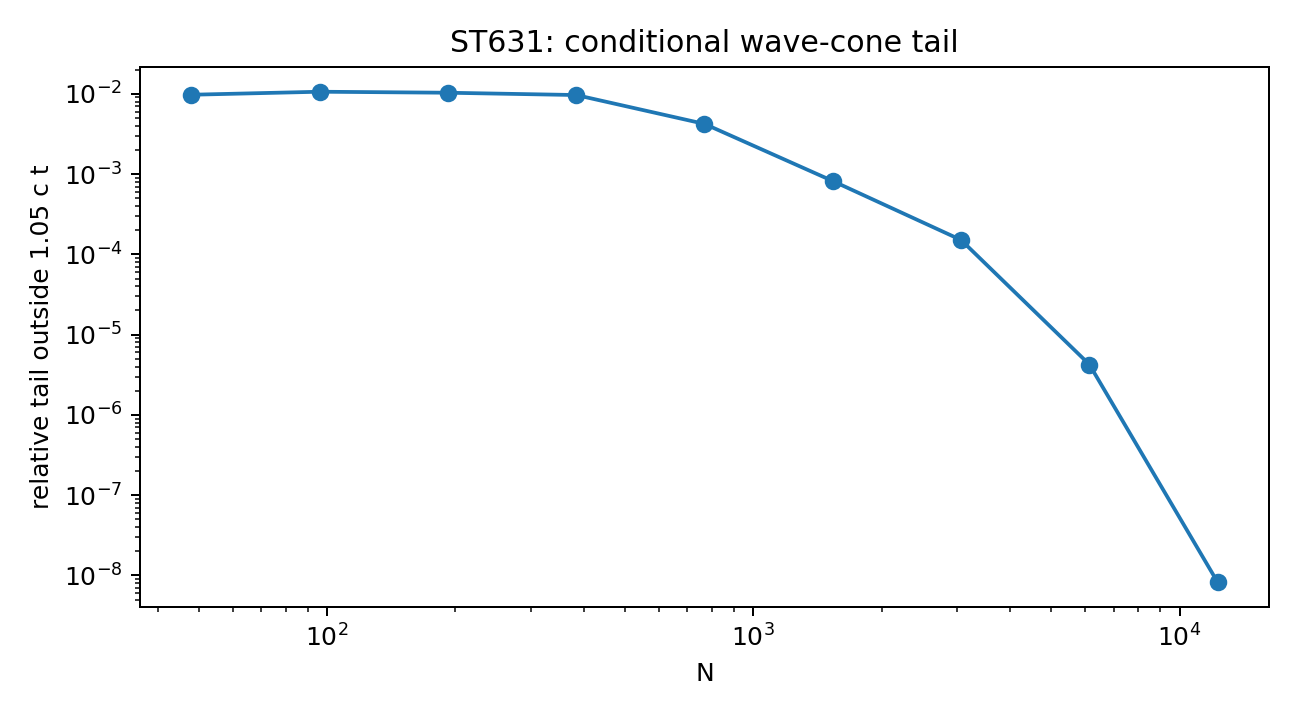
\includegraphics[width=.8\textwidth]{FIN_ST627_ST641_Figures/st631_wave_tail.png}\caption{Conditional zero-rate wave tails vanish toward a continuum cone.}\end{figure}

Under consistency and stability, the limiting scalar equation is
\[
\partial_T^2\phi-C\partial_x^2\phi=0,
\]
with exact $1+1$ domain of dependence speed $\sqrt C$. This is the shortest current mathematical path from FIN spatial weights to a causal wave equation.

It is conditional. The zero-rate tower, coordinate embedding, ballistic clock and calibration are not generated by $A_{12}$. Moreover a scalar $1+1$ equation does not supply $3+1$ isotropy, Lorentz boosts, Maxwell fields, photons or matter coupling.

\subsection{Round-VI ledger}
\begin{longtable}{@{}p{.09\textwidth}p{.32\textwidth}p{.49\textwidth}@{}}\toprule Program&Status&Result\\\midrule\endhead
ST627--629&\proven&Scaling exponents, one-clock no-go and two clock classes.\\
ST630&\proven&Rescaled dispersion converges to $Ck^2$.\\
ST631&\strong&Finite-lattice wave tails converge numerically toward zero.\\
ST632--633&\conditional&Continuum consistency and three functional calculi.\\
ST634&\proven&Duality survives; wave scaling separates.\\
ST635&\proven&Dimensionless speed plus one wave length/time anchor.\\
ST636&\conditional&Scalar continuum light-cone mechanism.\\
ST637&\proven&Light-cone slope is not Lorentz/light-field closure.\\
ST638&consolidated&No inevitability, but one coherent conditional bridge.\\
ST639--641&blocked&Independent frontiers, source package and evidence absent.\\\bottomrule\end{longtable}

\section{Falsification and obstruction ledger}
\begin{longtable}{@{}p{.29\textwidth}p{.29\textwidth}p{.33\textwidth}@{}}\caption{What failed and what follows.}\\\toprule Attempt&Result&Licensed conclusion\\\midrule\endfirsthead\toprule Attempt&Result&Licensed conclusion\\\midrule\endhead
Read $c$ directly from $C_{12}$&Formal, phase and group speeds disagree&No continuum speed at the endpoint.\\
Positive $d^{-1.8}$ refinement&Fractional exponent $0.8$&No finite nonzero low-$k$ wave speed.\\
Literal signed strict extension&Negative modes at $N=48$&Not a universal positive Laplacian refinement.\\
Coarse exact naturality&Continuous unbounded speed fiber&Complete coarse dynamics cannot identify fine speed.\\
$q_N\sim N^{-2}$ tower&Speed coefficient grows with depth&Per-layer finite contribution is not an infinite limit.\\
Polynomial antipodal locality&Exponential moment diverges&No uniform exponential cone from polynomial $q_N$.\\
One refinement clock&Requires both $z=2$ and $z=1$&At least two channel conversion classes.\\
Naive log interval chart&Negative Krawczyk margin&Method stop; numerical root not refuted.\\
Zero-rate local tower&Conditional PDE cone succeeds&Compatibility demonstrated, inevitability not.\\\bottomrule\end{longtable}

\section{Deepest interpretation after six rounds}
\claimbox{\textbf{Deepest surviving interpretation.} FIN's finite spectral core does not contain a unique speed of light. It contains enough structure to support a conditional local wave continuum once a refinement universality class, wave-clock scaling and calibration are selected. Exact coarse self-similarity hides rather than determines the fine propagation law.}

The internal-observer intuition is mathematically viable in the following form:
\[
c_n^{\rm phys}=\frac{\ell_n}{\tau_n}\widehat c_n
=c_*.
\]
But this equality is a constraint on three structures: the fine generator, the layer coordinate map and the calibration cocycle. A coarse observer may see identical dynamics while all three vary in the hidden fiber. Therefore constant internally measured $c$ is not sufficient to reconstruct the external/fractal layer law.

The result is simultaneously positive and negative:
\begin{itemize}
\item \textbf{Positive:} a precise conditional sequence reaches a scalar continuum cone.
\item \textbf{Negative:} current FIN does not select that sequence, one universal clock is impossible, and the observed SI value remains an anchor rather than a prediction.
\end{itemize}

\section{Recommended next cycle: ST642--ST656}
\begin{longtable}{@{}p{.08\textwidth}p{.30\textwidth}p{.51\textwidth}@{}}\caption{Ranked next studies.}\\\toprule Rank&Programme&Acceptance criterion\\\midrule\endfirsthead\toprule Rank&Programme&Acceptance criterion\\\midrule\endhead
1&ST642 zero-rate source theorem&Derive $q_N=0$ from a new strict locality/action principle, or prove no invariant principle in a declared class can do so.\\
2&ST643 Green--Schur locality selector&Test whether response-preserving compression plus uniform locality forces the zero tower.\\
3&ST644 continuum convergence theorem&Add stability and prove strong convergence of wave propagators, not only stencil consistency.\\
4&ST645 uniform tail certificate&Replace numerical tails by an analytic bound uniform in $N$ outside $(1+\epsilon)ct$.\\
5&ST646 $3+1$ isotropic refinement&Construct or obstruct an isotropic carrier family with quadratic symbol.\\
6&ST647 emergent Lorentz boosts&Test convergence of discrete energy-momentum transformations and quantify boost-breaking corrections.\\
7&ST648 gauge/light sector&Determine the additional bundle/connection data needed for Maxwell rather than a scalar wave.\\
8&ST649 two-clock operational protocol&Freeze preparations and records that independently identify ballistic and diffusive clocks.\\
9&ST650 independent ruler/clock anchor&Design a noncircular calibration test; defining the ruler through light is rejected.\\
10&ST651 long-range polynomial cone&Prove the sharp causal-tail exponent for the positive $d^{-1.8}$ class.\\
11&ST652 signed oscillatory Krein route&Classify whether an indefinite refinement has a stable causal interpretation without pretending it is Markov.\\
12&ST653 predictor-correlated IR intervals&Retain $z$--$b$ dependence symbolically to avoid the failed naive log interval.\\
13&ST654 transition/algebra state map&Reopen only with a genuinely new interval or characteristic-zero method.\\
14&ST655 strict source gate&Accept only a new formula-level refinement/clock/selector provider.\\
15&ST656 evidence gate&Accept only independently custodied laboratory records.\\\bottomrule\end{longtable}

\section{Final conclusions}
\begin{enumerate}
\item The fixed strict operator has no exact causal cone and does not by itself possess a continuum wave number.
\item A finite nonzero low-$k$ speed exists exactly for a quadratic generator symbol.
\item Positive $d^{-1.8}$ refinement is fractional; naive signed strict refinement loses positivity.
\item Exact dyadic refinement produces an unbounded fine-speed fiber invisible to every coarse spectral record.
\item Across a tower, finite speed requires $\sum N^2q_N<\infty$; uniform exponential locality is stricter.
\item Exact speed stationarity conditionally selects the zero-rate tower, but the stationarity law is not strict-sourced.
\item One clock cannot preserve unitary/heat and wave limits. Two channel-specific clock classes are minimally required.
\item The zero-rate finite-range tower conditionally converges to a scalar $1+1$ wave operator with a causal cone.
\item This does not derive the SI value of $c$, Lorentzian $3+1$ spacetime, Maxwell light, apparatus or experiment.
\item Current FIN therefore supports a mathematically coherent route to causal waves but not a unique or inevitable physical bridge.
\end{enumerate}

\appendix
\section{Reproducibility inventory}
The authoritative round outputs are
\begin{itemize}
\item \texttt{FIN\_ST552\_ST566\_Results.json},
\item \texttt{FIN\_ST567\_ST581\_Results.json},
\item \texttt{FIN\_ST582\_ST596\_Results.json},
\item \texttt{FIN\_ST597\_ST611\_Results.json},
\item \texttt{FIN\_ST612\_ST626\_Results.json},
\item \texttt{FIN\_ST627\_ST641\_Results.json},
\end{itemize}
with six Python sources, six test modules and figure directories. The combined suite passes 31 tests.

\section{Nonclaims}
This release does not complete legacy-to-strict, transfer legacy physical roles, discharge $QW$-2191, source gain/selector/units, derive a physical photon, Standard Model, gravity, $L_{\rm total}$ or ToE, or claim laboratory confirmation. All future research PDFs remain English.
\end{document}
